\documentclass[10pt,aspectratio=169]{beamer}

\usetheme{metropolis}
\usepackage{appendixnumberbeamer}

\usepackage{booktabs}
\usepackage[scale=2]{ccicons}
\usepackage[round]{natbib}
\usepackage{siunitx}

\usepackage{pgfplots}
\usepgfplotslibrary{dateplot}

\usepackage{tikz,ifthen}
\usetikzlibrary{arrows,shapes,positioning, calc, snakes}
\usetikzlibrary{decorations.markings, decorations.pathmorphing}
\tikzstyle arrowstyle=[scale=1]
\tikzstyle directed=[postaction={decorate,decoration={markings,
    mark=at position .65 with {\arrow[arrowstyle]{stealth}}}}]
\tikzstyle reverse directed=[postaction={decorate,decoration={markings,
    mark=at position .65 with {\arrowreversed[arrowstyle]{stealth};}}}]
\tikzset{wavy/.style={decorate, decoration={snake}, draw=olive}}
\def\layersep{2.5}

\usepackage{xspace}
\usepackage{changepage}
\newcommand{\themename}{\textbf{\textsc{metropolis}}\xspace}
\usepackage{csquotes}

\usepackage{amssymb,amsmath,amsthm}
\newcommand{\im}{ {i\!-\!1} }
\newcommand{\ip}{ {i\!+\!1} }
\newcommand{\T}{\mathrm{T}}
\newcommand{\R}{\mathrm{R}}
\newcommand{\dd}{\mathrm{d}}

\usepackage{textcomp}
\graphicspath{{../fig/}}

\title{Self-sustained probabilistic computing on spike-based neuromorphic systems}
\date{ Bernstein Conference, September 29th - October 2nd, 2020}
\author{ \footnotesize{ \textbf{A.~F.~Kungl\textsuperscript{1,2}}, D.~Dold\textsuperscript{1,2}, A.~Baumbach\textsuperscript{1,2}, S.~Schmitt\textsuperscript{1}, J.~Kl\"ahn\textsuperscript{1}, N.~G\"urtler\textsuperscript{1}, P.~M\"uller\textsuperscript{1},  A.~Kugele\textsuperscript{1}, L.~Leng\textsuperscript{1,2}, E.~M\"uller\textsuperscript{1}, C.~Koke\textsuperscript{1}, M.~Kleider\textsuperscript{1}, C.~Mauch\textsuperscript{1}, O.~J.~Breitwieser\textsuperscript{1}, M.~G\"uttler\textsuperscript{1}, D.~Husmann\textsuperscript{1}, K.~Husmann\textsuperscript{1}, A.~Hartel\textsuperscript{1}, V.~Karasenko\textsuperscript{1},  J.~Ilmberger\textsuperscript{1}, A.~Gr\"ubl\textsuperscript{1},  J.~Schemmel\textsuperscript{1}, K.~Meier\textsuperscript{1}, M.~A.~Petrovici\textsuperscript{1,2} }} % Author(s)

\institute{\small \textsuperscript{1}Heidelberg University, Kirchhoff-Institute for Physics; \textsuperscript{2}University of Bern, Institute for Physiology}

\newcommand\blfootnote[1]{%
  \begingroup
  \renewcommand\thefootnote{}\footnote{#1}%
  \addtocounter{footnote}{-1}%
  \endgroup
}


\begin{document}

\maketitle

\begin{frame}{Probabilistic models\blfootnote{\cite{berkes2011spontaneous,orban2016neural}}}

\begin{columns}[c]
    \column{0.65\textwidth}
    \begin{center}
        \includegraphics[width=0.7\textwidth]{example-image-a}
    \end{center}

    \column{0.35\textwidth}
    \begin{center}
        \begin{itemize}
            \item
            neural activity is inherently noisy
            \item
            noisiness is interpreted as a probabilistic computation
        \end{itemize}
    \end{center}

\end{columns}


\end{frame}

\begin{frame}{Sampling with spiking neurons \blfootnote{\cite{petrovici2016stochastic}}}

\begin{columns}
    \column{0.65\textwidth}
    \begin{center}
        \includegraphics[width=1.0\textwidth]{figTHfull}
    \end{center}

    \column{0.35\textwidth}
        \begin{itemize}
            \item
            interpreting dynamics as sampling
            \item
            spikes define the state
            \item
            useful for neuromorphic hardware
        \end{itemize}

\end{columns}

\vspace{0.5cm}



\end{frame}


\begin{frame}{Sampling with deterministic neurons\blfootnote{\cite{dold2019stochasticity}}}

\begin{columns}[c]
    \column{0.65\textwidth}
    \begin{center}
        \includegraphics[width=0.7\textwidth]{example-image-a}
    \end{center}

    \column{0.35\textwidth}
    \begin{center}
        \begin{itemize}
            \item
            no need for explicit noise
            \item
            independent functional networks feed each other with noise
        \end{itemize}
    \end{center}

\end{columns}



\end{frame}


\begin{frame}{The BrainScaleS-1 neuromorphic system \blfootnote{\cite{schemmel2010wafer}}}

\begin{columns}
    \column{0.60\textwidth}
    \begin{center}
        \includegraphics[width=0.99\textwidth]{figHWfull.pdf}
    \end{center}

    \column{0.40\textwidth}
    \begin{center}
        \begin{itemize}
            \item
            mixed-analog signal hardware
            \item
            200k neurons and 40 million synapses
            \item
            \num{e4}-fold acceleration
        \end{itemize}
    \end{center}

\end{columns}


\end{frame}

\begin{frame}{Application on neuromorphic hardware \blfootnote{\cite{kungl2019accelerated}}}

\begin{columns}
    \column{0.6\textwidth}
    \begin{center}
        \only<1>{\includegraphics[width=0.9\textwidth]{figInference.pdf}}
        \only<2>{\includegraphics[width=0.7\textwidth]{figPatternComp.pdf}}
    \end{center}

    \column{0.4\textwidth}
    \begin{center}
        \begin{itemize}
            \item
            in-the-loop training
            \item
            inference, pattern completion and data generation
            \item
            \num{2e5} images per second throughput
        \end{itemize}
    \end{center}

\end{columns}


\end{frame}


\begin{frame}{Outlook and ongoing work\blfootnote{\cite{czischek2020spiking}}}

\begin{columns}
    \column{0.6\textwidth}
    \begin{center}
        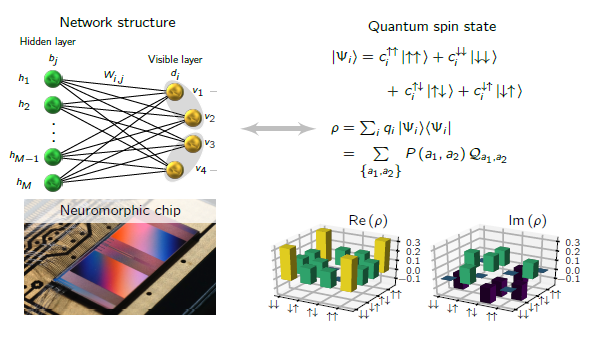
\includegraphics[width=1.0\textwidth]{quantumhw.png}
    \end{center}

    \column{0.4\textwidth}
    \begin{center}
        \begin{itemize}
            \item
            quantum many-body problems
            \item
            spike-based on-chip learning
            \item
            connection to experiments
        \end{itemize}
    \end{center}

\end{columns}

\end{frame}

\begin{frame}{People behind the publications}

\begin{columns}
    \column{0.6\textwidth}
    \begin{center}
        
        
\includegraphics[width=0.95\textwidth]{visions.jpg}
    \end{center}
        \vspace{0.05cm}
    \begin{center}
        \def \myHeight {0.12}
        
\includegraphics[height=\myHeight\textheight]{logos/eu.png}
        
\includegraphics[height=\myHeight\textheight]{logos/hbp.png}
        
\includegraphics[height=\myHeight\textheight]{logos/kip.png}
        
\includegraphics[height=\myHeight\textheight]{logos/logo_bern.png}
        
\includegraphics[height=\myHeight\textheight]{logos/logo_staerk.png}
        
\includegraphics[height=\myHeight\textheight]{logos/uhei.png}
        
\includegraphics[height=\myHeight\textheight]{logos/visions.png}
        %
\includegraphics[width=1.0\textwidth]{visions.png}
    \end{center}

    \column{0.4\textwidth}
    \begin{center}
        \textbf{Contact us to get access to the hardware!} \\
        \vspace{0.5cm}
        \url{https://www.humanbrainproject.eu/en/silicon-brains}
    \end{center}

\end{columns}

\end{frame}




\begin{frame}[allowframebreaks]
        \frametitle{References}
        \bibliographystyle{plainnat}
        \bibliography{../bib.bib}
\end{frame}


\end{document}






\begin{frame}{Defining equations}

    \textbf{The Lagrange function:}
    \begin{equation}
        L = \underbrace{\frac{1}{2} \sum_{i=1}^{N} \left \Vert u_i - W_i \bar r _{i-1}\right \Vert ^2}_{\text{prediction error}} + \underbrace{\frac{\beta}{2} \left \Vert u_N - y_N \right \Vert ^2}_{\text{cost function}}
    \end{equation}

    \textbf{Future discounted membrane potential}
    \begin{equation}
        \tilde{u} (t) = \frac{1}{\tau} \int_t^\infty u(\hat t) \exp \left (-\frac{\hat t - t}{\tau} \right ) \mathrm{d}\hat t
    \end{equation}

    \textbf{And applying the Euler-Lagrange equations to $E$ with $\tilde u$:}
    \begin{equation}
        \frac{\partial L}{\partial \tilde{u}} = \frac{\mathrm{d}}{\mathrm{d}t} \frac{\partial L}{\partial \dot{\tilde{u}}}
    \end{equation}

\end{frame}

\begin{frame}{Dynamics and backpropagation}

\begin{columns}
    \column{0.49\textwidth}
    \textbf{The obtained dynamics}
    \begin{align}
        \tau \dot{u_i} &= -u_i + W_i r_{i-1} + e_i\,, \\
r_i &= \underbrace{\bar{r}_i + \tau \dot{\bar{r}}_i}_\text{look-ahead spiking}\,, \hspace{4mm} e_i = \bar{e}_i + \tau \dot{\bar{e}}_i \,, \\
\bar{e}_i &= \underbrace{\bar{r_i}' \odot W_{i+1}^\mathrm{T} (u_{i+1} - W_{i+1}\bar{r_i})}_\text{error backprop}\,, \\ 
\bar{e}_N &= \underbrace{\beta(y_N - u_N)}_\text{nudging}\,,             
    \end{align}
    \textbf{The plasticity}
    \begin{align}
        \dot{W_i} = - \eta \frac{\partial E}{\partial W_i} = \eta (u_i - W_i \bar r_{i-1} ) \bar r_{i-1}^T
    \end{align}

    \column{0.49\textwidth}
    \textbf{How do we see the backprop?} \\
    Low-pass filter equation of motion
    \begin{equation*}
        \bar e_i = u_i - W_{i+1} \bar r_i
    \end{equation*}
    and realize
    \begin{equation*}
        \bar e_i = \bar{r_i}' \odot W_{i+1}^\mathrm{T} \underbrace{(u_{i+1} - W_{i+1}\bar{r_i})}_{\bar e_{i+1}}
    \end{equation*}
    hence \textbf{ecce backprop}
    \begin{align*}
        \bar e_i &= \bar{r_i}' \odot W_{i+1}^\mathrm{T} \bar e_{i+1} \\
        \bar e_N &= \beta(y_N - u_N) 
    \end{align*}

\end{columns}


\end{frame}

\begin{frame}{What microcircuits?}

    \begin{columns}
        \column{0.39\textwidth}
            \begin{itemize}
                \item
                Local structure between layers
                \item
                Propagates error to deeper layers
                \item
                local predictive coding
            \end{itemize}

        \column{0.60\textwidth}

        \begin{center}
            \includegraphics[height=1.0\textheight]{figs/microcircuit.png}
        \end{center}
    \end{columns}

\end{frame}


\begin{frame}{In Application}

    \begin{center}
        \includegraphics[width=1.05\textwidth]{figs/fig4_tikz.pdf}
    \end{center}
    
\end{frame}


\begin{frame}{Learning the interneurons and the feedback}

The feedback weights $B$ should minimize the corresponding energy:
\begin{align}
    \dot{B}_l &= \eta_B (\bar{r}^P_l - B_l u_{l+1})u_{l+1}^T \\
    E_b^{(l)} &= \left \Vert \bar{r}_l^P - B_l W_{l+1} \bar{r}^P_l \right \Vert^2
\end{align}
The $B$ should approximately converge to the pseudo-inverse of the forward weights $W^+$. \\
\vspace{1cm}
Learning the interneurons:
\begin{align}
    \dot{W}^{IP} &= \eta_{IP}(u_l^I - W^{IP}\bar{r}_l^P)(\bar{r}_l^P)^T \\
    \dot{W}^{PI} &= \eta_{PI}(B_l u_{l+1} - W^{PI}\bar{r}_l^I)(\bar{r}_l^I)^T\\
    E_I^{(l)} &= \left \Vert B_l W_{l+1} \bar{r}_l - W_{l}^{PI} W_{l}^{IP} \bar{r}_l  \right \Vert^2 
\end{align}
That is going a round over the pyramidal neurons ($B_l W_{l+1}$) should yield the same as going over the interneurons ($W_{l}^{PI} W_{l}^{IP}$).\\
Hence, it should work but...\dots
\end{frame}

\begin{frame}{Setup}

\begin{columns}[c, onlytextwidth]
    \column{0.49\textwidth}
    \begin{itemize}
        \item
        Three layered network: input-hidden-label
        \item
        no feed-forward learning
        \item
        no nudging at the label neurons
        \item
        $B$ and interneurons learn in the setup
    \end{itemize}

    \column{0.49\textwidth}
    \begin{center}
        \includegraphics[width=1.0\textwidth]{figs/network.pdf}
    \end{center}
    

\end{columns}


\end{frame}


\begin{frame}{If the learning rates are equal then $B$ dominates}
        \begin{center}
            \includegraphics[width=1.0\textwidth]{figs/equal_etas.png}
        \end{center}
\end{frame}

\begin{frame}{If only the interneurons learn then it almost works}
        \begin{center}
            \includegraphics[width=1.0\textwidth]{figs/onlyI.png}
        \end{center}
\end{frame}

\begin{frame}{If the interneurons start from self-predicting state then it seems to work}
        \begin{center}
            \includegraphics[width=1.0\textwidth]{figs/fromSelfPred.png}
        \end{center}
\end{frame}

\begin{frame}{Current best guess}
        \begin{center}
            \includegraphics[width=1.0\textwidth]{figs/bestGuess.png}
        \end{center}
\end{frame}

\begin{frame}{Current best guess if only the interneurons learn}
        \begin{center}
            \includegraphics[width=1.0\textwidth]{figs/onlyIBest.png}
        \end{center}
\end{frame}


\begin{frame}{Conclusion and Outlook}

\textbf{Our goal}
    \begin{itemize}
        \item
        See $E_b$ and $E_I$ sink in the same experiment
        \item
        If finished then finalize the publication
    \end{itemize}

\textbf{Question}
    \begin{itemize}
        \item
        What can we still tune to achieve the goal?
        \item
        What do we do if the goal stays elusive?
    \end{itemize}

\end{frame}






\begin{tikzpicture}[shorten >=1pt,->,draw=black!50, node distance=\layersep]
    \tikzstyle{every pin edge}=[<-,shorten <=1pt]
    \tikzstyle{neuron}=[circle,fill=black!25,minimum size=17pt,inner sep=0pt]
    \tikzstyle{input neuron}=[neuron, fill=green!50];
    \tikzstyle{output neuron}=[neuron, fill=red!50];
    \tikzstyle{hidden neuron}=[neuron, fill=blue!50];
    \tikzstyle{annot} = [text width=4em, text centered]

    % Draw the input layer nodes
    \foreach \name / \y in {1,...,4}
    % This is the same as writing \foreach \name / \y in {1/1,2/2,3/3,4/4}
        \node[input neuron, pin=left:Input \#\y] (I-\name) at (0,-\y) {};

    % Draw the hidden layer nodes
    \foreach \name / \y in {1,...,5}
        \path[yshift=0.5cm]
            node[hidden neuron] (H-\name) at (\layersep,-\y cm) {};

    % Draw the output layer node
    \node[output neuron,pin={[pin edge={->}]right:Output}, right of=H-3] (O) {};

    % Connect every node in the input layer with every node in the
    % hidden layer.
    \foreach \source in {1,...,4}
        \foreach \dest in {1,...,5}
            \path (I-\source) edge (H-\dest);

    % Connect every node in the hidden layer with the output layer
    \foreach \source in {1,...,5}
        \path (H-\source) edge (O);

    % Annotate the layers
    \node[annot,above of=H-1, node distance=1cm] (hl) {Hidden layer};
    \node[annot,left of=hl] {Input layer};
    \node[annot,right of=hl] {Output layer};
\end{tikzpicture}
